\documentclass[sigconf,anonymous,review]{acmart}
\settopmatter{printacmref=false,printfolios=true}
\setcopyright{none}
\renewcommand\footnotetextcopyrightpermission[1]{}
\acmConference[ICCRD 2027]{2027 19th International Conference on Computer Research and Development}{January 15--17, 2027}{Singapore}
\usepackage{mathtools}
\usepackage{booktabs,tabularx,array}
\usepackage{graphicx}
\usepackage{microtype}
\usepackage{balance}
\setlength{\emergencystretch}{1em}
\begin{document}
\title[HDA-NQ for Probabilistic Time Series Forecasting]
{HDA-NQ: Horizon-Conditioned Deformable Attention with Non-Crossing Quantiles for Long-Term Probabilistic Time Series Forecasting}
\begin{abstract}
Long-term probabilistic time series forecasting aims to quantify future uncertainty while maintaining forecasting accuracy. However, the temporal dependencies between historical observations and future time steps may vary across forecasting horizons. Existing direct multi-step forecasting methods typically map historical inputs to future outputs without explicitly adapting historical feature retrieval to individual forecasting horizons. Moreover, conventional quantile regression without ordering constraints may suffer from quantile crossing, leading to inconsistent prediction intervals. To address these problems, this paper investigates horizon-aware temporal feature extraction and non-crossing quantile regression, and proposes a unified probabilistic forecasting framework (HDA-NQ) that integrates horizon-conditioned deformable attention with non-crossing quantile regression. Through learnable sampling offsets and sparse attention aggregation, the proposed framework adaptively extracts relevant historical temporal features for different forecasting horizons, enabling horizon-specific temporal representation learning. A gated historical correction mechanism is further employed to enhance the ability of the model to capture local temporal dynamics. In addition, a median-anchored quantile regression strategy is developed by parameterizing the differences between adjacent quantiles as positive values, thereby ensuring the monotonicity of predicted quantiles and avoiding quantile crossing. Across 17 completed dataset--horizon settings on five benchmark datasets, HDA-NQ attains the lowest mean pinball loss in 15 settings against four quantile-adapted forecasting backbones. Component experiments support horizon conditioning and learned sampling at the studied settings, while empirical interval coverage remains below nominal levels.
\end{abstract}
\ccsdesc[500]{Computing methodologies~Machine learning}
\ccsdesc[300]{Information systems~Data mining}
\keywords{Deformable attention, Non-crossing quantile regression, Probabilistic forecasting, Long-term time series forecasting}
\maketitle

\section{Introduction}

With the development of deep learning, data-driven methods have been widely applied to object detection~\cite{vidal2026hybrid}, energy forecasting~\cite{abisoye2024solar}, and financial analysis~\cite{krawczyk2025financial} owing to their feature extraction and nonlinear modeling capabilities. In time series forecasting, extracting informative features from historical observations and capturing complex temporal dependencies are essential for improving forecasting performance. However, conventional deterministic forecasting methods only provide point estimates of future observations and cannot adequately characterize predictive uncertainty. In contrast, probabilistic forecasting estimates conditional quantiles or predictive distributions to provide richer information about future uncertainty, thereby supporting risk assessment and decision-making~\cite{chen2025noncrossing}. Therefore, improving forecasting accuracy while effectively quantifying future uncertainty remains an important research problem in long-term time series forecasting.

In recent years, considerable progress has been made in long-term time series forecasting. Representative methods, including DLinear~\cite{zeng2023transformers}, PatchTST~\cite{nie2023timeseries}, iTransformer~\cite{liu2024itransformer}, and TimeMixer~\cite{wang2024timemixer}, have demonstrated the effectiveness of linear modeling, patch-based representation learning, cross-variate dependency modeling, and multiscale feature extraction. Meanwhile, probabilistic forecasting models such as DeepAR~\cite{salinas2020deepar}, the multi-horizon quantile recurrent forecaster~\cite{wen2017multihorizon}, and the Temporal Fusion Transformer~\cite{lim2021temporal} provide effective approaches to uncertainty quantification in time series forecasting.

Despite these advances, two issues remain worth investigating in long-term probabilistic time series forecasting. First, time series generally contain multiple temporal patterns, including trends, periodic fluctuations, and local variations. Different future time steps may therefore exhibit heterogeneous dependencies on historical observations. However, many existing direct multi-step forecasting methods generate future predictions from shared historical representations without explicitly adjusting historical sampling positions for individual forecasting steps. Second, quantile regression provides a flexible non-parametric approach to probabilistic forecasting~\cite{koenker1978regression}, but unconstrained quantile estimation may lead to quantile crossing, resulting in inconsistent prediction intervals. How to improve temporal feature extraction while maintaining quantile monotonicity remains an important issue in long-term probabilistic forecasting.

To address these issues, this paper proposes a unified probabilistic forecasting framework that integrates horizon-conditioned deformable attention with non-crossing quantiles (HDA-NQ). Specifically, a horizon-conditioned deformable attention mechanism is developed to adaptively extract relevant historical features through horizon-specific queries, learnable sampling offsets, and sparse attention aggregation. A gated historical correction mechanism is introduced to enhance the modeling of local temporal dynamics. Furthermore, a median-anchored non-crossing quantile regression strategy is employed to ensure the monotonicity of predicted quantiles through positive-gap parameterization.

The main contributions of this paper are summarized as follows:

\begin{itemize}

\item A horizon-conditioned deformable attention mechanism is proposed for long-term probabilistic time series forecasting. By combining horizon-specific queries with learnable sampling offsets, the proposed mechanism adaptively retrieves relevant historical features and captures horizon-specific temporal dependencies.

\item A unified probabilistic forecasting framework integrating gated historical correction and median-anchored non-crossing quantile regression is developed. The framework enhances the modeling of local temporal dynamics and ensures quantile monotonicity through positive-gap parameterization without requiring post-processing.

\item The proposed HDA-NQ achieves favorable probabilistic forecasting performance across multiple benchmark datasets and forecasting lengths. Comparative experiments and ablation studies further demonstrate the effectiveness of the proposed forecasting framework and its key components.

\end{itemize}

\section{Related Work}
\label{sec:related_work}

\paragraph{Probabilistic forecasts and quantile ordering.}
Quantile regression estimates conditional distributional information through an asymmetric absolute-error objective~\cite{koenker1978regression}. Calibration and sharpness jointly determine forecast quality~\cite{gneiting2007probabilistic}; proper scoring rules and interval scores assess complementary aspects of that quality~\cite{gneiting2007scoring,winkler1972decision}. DeepAR learns autoregressive predictive distributions across related series~\cite{salinas2020deepar}, whereas the Temporal Fusion Transformer directly produces quantiles for multiple future steps~\cite{lim2021tft}. Cannon's monotone composite quantile regression network guarantees non-crossing nonlinear quantiles~\cite{cannon2018noncrossing}. Our positive-gap head adopts structural ordering within this established line of work; its empirical calibration is evaluated separately.

\paragraph{Temporal representations.}
The Transformer provides a general sequence architecture based on attention~\cite{vaswani2017attention}. PatchTST combines temporal patches with encoder weights shared across variables~\cite{nie2023patchtst}. RevIN removes instance location and scale before prediction and restores them afterward~\cite{kim2022revin}. HADT-NQ adopts overlapping patches, shared temporal encoding, and non-affine RevIN. Simple direct linear forecasters can also be competitive~\cite{zeng2023dlinear}, motivating our linear control. Informer provides a long-sequence forecasting architecture and the requested provenance citation for the ETT datasets~\cite{zhou2021informer}.

\paragraph{Deformable attention.}
Deformable DETR learns offsets around reference points and attends to a sparse set of sampled features~\cite{zhu2021deformable}. DeformTime applies deformable attention to multivariable forecasting through variable and temporal operations~\cite{shu2025deformtime}. Thus, deformable forecasting attention and monotone quantile estimation both precede this work. HADT-NQ studies their combination for direct marginal forecasts: pooled history and a future-step embedding determine bounded temporal offsets, and interpolated keys and values supply each query's representation. Its independent processing of variables differs from DeformTime's focus on variable dependencies.

\paragraph{Comparison scope.}
Local comparators share a quantile objective and ordered head. Linear-NQ uses an affine map to raw output parameters; Patch-NQ projects encoded patches directly; Dense-NQ attends to all historical tokens; and Fixed-NQ disables learned offsets. These are local quantile controls, distinct from official DLinear or PatchTST implementations. The dense and fixed-reference controls isolate decoder behavior while retaining the shared temporal representation. Repeated experiments use ETTh1 and ETTh2 with three seeds; a separate Traffic case tests high-dimensional execution and marginal forecasting.

\section{Method}
\label{sec:method}

\subsection{Task, Normalization, and Patches}
Given history $X\in\mathbb R^{B\times L\times C}$, the model predicts
$\widehat Q\in\mathbb R^{B\times H\times C\times7}$ at levels
$\mathcal T=\{.05,.10,.25,.50,.75,.90,.95\}$.
A per-variable global scaler is fitted only on training observations. Model-side non-affine RevIN~\cite{kim2022revin} then normalizes each observed window:
\begin{equation}
 \widetilde X_{btc}=(X_{btc}-\mu_{bc})/s_{bc},\qquad
 s_{bc}=\sqrt{\operatorname{Var}_t(X_{btc})+10^{-5}}.
\end{equation}
Window statistics are detached from the gradient graph and use no future targets.

Length-$P$ patches at stride $S$ yield
$N=\lfloor(L-P)/S\rfloor+1$ historical tokens. An affine $P\rightarrow D$ projection and learned position embeddings form $T\in\mathbb R^{BC\times N\times D}$. Batch and variable axes are flattened, so variables share weights but do not exchange observations. With $L=336$, $P=16$, and $S=8$, $N=41$; the working width is $D=64$.

\subsection{Lightweight Historical Encoder}
Each residual token-wise MLP block computes
\begin{equation}
 T'=T+\operatorname{Drop}\!\left(W_2
 \operatorname{Drop}(\operatorname{GELU}(W_1\operatorname{LN}(T)))\right).
\end{equation}
The feature widths are $64\rightarrow128\rightarrow64$, followed after the block stack by a final layer normalization. These blocks mix features within each patch, not patch positions. Cross-patch information enters through historical pooling, decoder retrieval, and the direct correction branch.

The final configuration uses two blocks. This design retains a lightweight feature extractor while assigning history-wide retrieval to the decoder and the direct correction branch. Figure~\ref{fig:architecture} summarizes the forecasting path and its main components. Variables share model weights and are processed independently; the sampling illustrations are schematic rather than measured attention.

\begin{figure*}[t]
\centering
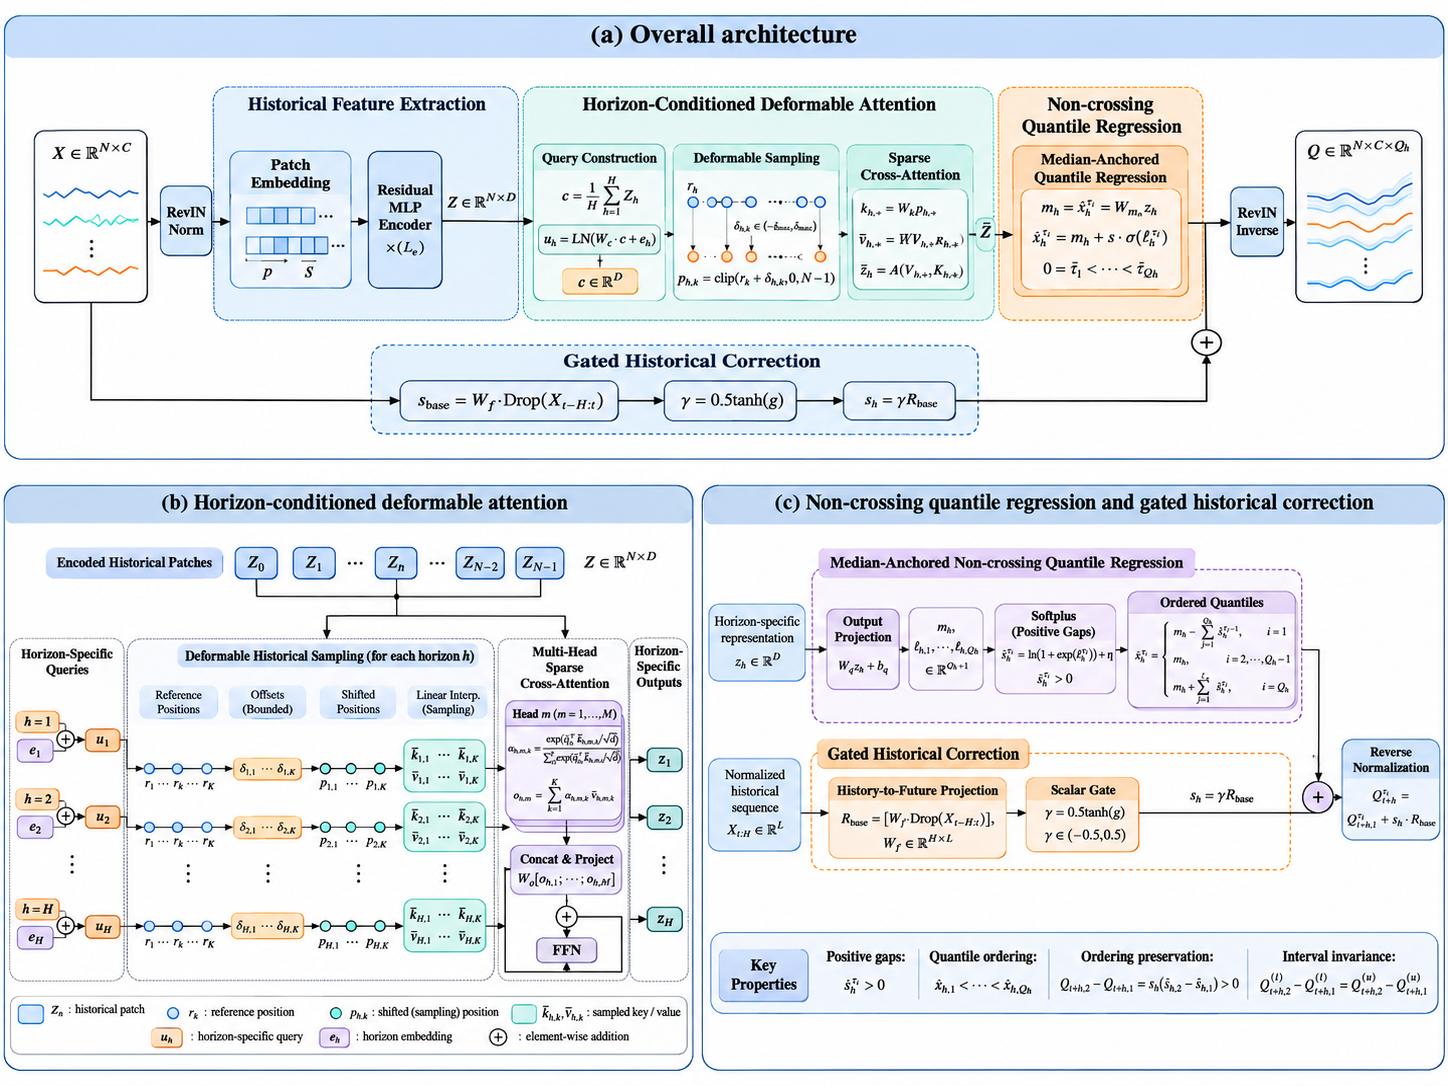
\includegraphics[width=.98\textwidth]{figures/architecture_draft.png}
\caption{Overall architecture of HDA-NQ.}
\Description{A forecasting path and an expanded decoder show normalization, patches, residual MLP encoding, future-step queries, sparse interpolation, attention, ordered quantiles, and a common history correction.}
\label{fig:architecture}
\end{figure*}

\subsection{Horizon-Conditioned Deformable Retrieval}
Suppressing batch and variable indices, let $Z\in\mathbb R^{N\times D}$ be encoded history. Future step $h$ receives a learned embedding $e_h$ and a history-conditioned query base:
\begin{equation}
 u_h=\operatorname{LN}\!\left(W_c\,N^{-1}\sum_nZ_n+e_h\right).
 \label{eq:query}
\end{equation}
For head $m$ and sample $k$, predicted offsets adjust uniform reference positions:
\begin{equation}
 \begin{aligned}
 r_k&=(k-1)(N-1)/(K-1),\\
 \delta_{hmk}&=a\tanh([W_\delta u_h]_{mk}),\\
 p_{hmk}&=\operatorname{clip}(r_k+\delta_{hmk},0,N-1).
 \end{aligned}
 \label{eq:offset}
\end{equation}
The configuration uses $M=8$ heads, $K=8$ samples, and $a=1.5$ patch tokens. Offset projections start at zero. The grid spans the whole history, but each sample moves only within a bounded neighborhood; sampling is not unrestricted global relocation. Clipping can hold endpoint samples at the boundary. In particular, the interpolation neighbors coincide at the rightmost reference; its zero-initialized offset receives no interpolation gradient and retains the most recent patch as an endpoint anchor.

Queries, keys, and values are affine projections of $u_h$ and $Z$, split into heads of width $d=D/M$. For either projected history $F$, a continuous location $p$ is sampled by
\begin{equation}
 \mathcal I(F,p)=(1-\lambda)F_\ell+\lambda F_r,\quad
 \ell=\lfloor p\rfloor,\ r=\min(\ell+1,N-1),\
 \lambda=p-\ell.
\end{equation}
Only neighboring features are gathered. Attention is normalized over the sampled locations within each head:
\begin{align}
 \alpha_{hmk}&=\operatorname{softmax}_k
 \left(q_{hm}^{\mathsf T}\mathcal I(K_m,p_{hmk})/\sqrt d\right),\\
 o_{hm}&=\sum_k\alpha_{hmk}\mathcal I(V_m,p_{hmk}).
\end{align}
The combined heads undergo residual refinement:
\begin{align}
 v_h&=\operatorname{LN}_1\!\left(u_h+\operatorname{Drop}(W_O[o_{h1};\ldots;o_{hM}])\right),\\
 z_h&=v_h+\operatorname{Drop}(\operatorname{FFN}(\operatorname{LN}_2(v_h))).
\end{align}
The decoder FFN has widths $D\rightarrow2D\rightarrow D$. Queries do not access future targets or attend to other future queries. Horizon chunking changes memory use without changing these dependencies.

\subsection{Ordered Outputs and Common Correction}
An affine projection of $z_h$ produces median $m_h$ and six gap logits. Positive gaps
$g^\pm_{hj}=\operatorname{softplus}(a^\pm_{hj})+\eta$,
$j=1,2,3$, $\eta=10^{-4}$, define
\begin{equation}
 \widetilde q_{h,4}=m_h,\qquad
 \widetilde q_{h,4\pm j}=m_h\pm\sum_{i=1}^jg^\pm_{hi}.
 \label{eq:ordering}
\end{equation}
Indices follow ascending quantile levels; negative-side cumulative outputs are reversed into ascending order. Reverse RevIN returns
$Q^{base}_{bhcq}=s_{bc}\widetilde q_{bhcq}+\mu_{bc}$.

A direct history correction is added to the base output:
\begin{equation}
 \begin{aligned}
 R_{bhc}&=[W_R\operatorname{Drop}(\widetilde X_{b,:,c})]_h,\\
 \gamma&=0.5\tanh(g),\\
 \widehat Q_{bhcq}&=Q^{base}_{bhcq}+s_{bc}\gamma R_{bhc}.
 \end{aligned}
 \label{eq:correction}
\end{equation}
Here $W_R\in\mathbb R^{H\times L}$ has no bias and starts at zero; the gate starts at $\gamma=0.1$. The bounded gate does not bound correction amplitude because $W_R$ is trainable. The same correction shifts every quantile, supplying a direct history-to-future path without changing interval widths for fixed base outputs.

\noindent\textbf{Ordering property.}
Adjacent cumulative outputs in Eq.~\eqref{eq:ordering} differ by a positive gap. Multiplication by $s_{bc}>0$, addition of $\mu_{bc}$, and the common shift in Eq.~\eqref{eq:correction} preserve their order. In floating-point computation, rounding may produce ties. Ordering establishes neither nominal coverage nor simultaneous uncertainty across variables and future steps.

\subsection{Objective and Computational Scope}
All working configurations minimize mean pinball loss:
\begin{equation}
 \begin{aligned}
 \mathcal L&=\frac{1}{7BHC}\sum_{b,h,c,q}
 \max\{\tau_q e_{bhcq},(\tau_q-1)e_{bhcq}\},\\
 e_{bhcq}&=Y_{bhc}-\widehat Q_{bhcq}.
 \end{aligned}
\end{equation}
No difference auxiliary loss or post-hoc calibration is used. With $K<N$, sampled attention scores and aggregation cost $O(BCHKD)$ rather than $O(BCHND)$ for dense historical attention. This comparison excludes projections, FFNs, the encoder, and the $O(BCLH)$ history correction. It therefore does not imply lower end-to-end latency; no hardware speedup claim is made.

\section{Experiments}
\label{sec:experiments}

\subsection{Datasets and Evaluation Protocol}
This revision reports 315 completed test runs across seven benchmark datasets and 21 dataset--horizon settings. Each displayed setting contains five models and three seeds. Other settings in the seven-dataset protocol remain in progress and are excluded until complete. Table~\ref{tab:data} describes the datasets represented by these comparisons.

All reported comparisons use $L=336$ and independently trained models for the reported $H\in\{96,192,336,720\}$. Forecasts are not obtained by truncating a longer prediction. ETT originates from the benchmark of Zhou et al.~\cite{zhou2021informer}; hourly and 15-minute observations have different physical forecast durations. All reported settings are long-term forecasting tasks.

\begin{table}[t]
\centering\small
\caption{Datasets represented in the completed comparisons.}
\label{tab:data}
\begin{tabular*}{\linewidth}{@{\extracolsep{\fill}}lrrl@{}}
\toprule
Dataset & Rows & Variables & Split \\
\midrule
ETTh1 & 17,420 & 7 & 60/20/20 \\
ETTh2 & 17,420 & 7 & 60/20/20 \\
ETTm1 & 69,680 & 7 & 60/20/20 \\
ETTm2 & 69,680 & 7 & 60/20/20 \\
Traffic & 17,544 & 862 & 70/10/20 \\
Weather & 52,696 & 21 & 70/10/20 \\
Electricity & 26,304 & 321 & 70/10/20 \\
\bottomrule
\end{tabular*}
\end{table}


Scalers are fitted on training rows only. Future targets remain within their assigned split; validation and test inputs may contain earlier observed history. No future covariates or calendar features are supplied. The ETT ratio split differs from common fixed-month protocols, so published scores from other partitions are not imported. Full-test metrics cover every eligible window and variable. Overlapping windows contribute to forecast scores but are not treated as independent statistical replicates.

\subsection{Baselines and Controlled Variants}
The backbones are DLinear~\cite{zeng2023transformers}, PatchTST~\cite{nie2023timeseries}, TimeMixer~\cite{wang2024timemixer}, and iTransformer~\cite{liu2024itransformer}. We retain each point prediction backbone and append the same median and positive-gap parameterization to each scalar forecast. All train end-to-end with pinball loss. The suffix \emph{-NQ} identifies this adaptation, not an original probabilistic result from the cited paper. These heads share a construction, but their scalar inputs differ from HDA-NQ's decoder features; parameter budgets and representational capacities are not equal.

The final-structure removals retain HDA-NQ settings apart from the specified component:
\begin{itemize}
\item \textbf{Fixed}: offsets are zero, while horizon queries and attention over the reference grid remain.
\item \textbf{Shared}: all future steps share one learned horizon embedding, retaining historical context.
\item \textbf{Dense}: cross-attention uses all historical patches, retaining query and residual refinement.
\item \textbf{No correction}: the direct historical correction is removed.
\item \textbf{Fixed + no correction}: both changes are applied, completing the offset--correction comparison.
\item \textbf{Independent}: seven unconstrained affine outputs replace the ordered head.
\end{itemize}
Each variant is retrained on ETTh1 at $H=96$ and $720$ with three seeds. The shared-query variant can still vary across steps through the direct correction; identical entire-model predictions are not implied. Independent outputs are evaluated with pinball and crossing rate; unordered endpoints are not reported as valid central intervals.

\subsection{Training and Validation Selection}
Training uses PyTorch 2.7.1, CUDA 12.8, and NVIDIA RTX 5090 GPUs in the \texttt{djjTF} environment. AdamW~\cite{loshchilov2019adamw} minimizes pinball loss, with gradient clipping at 1.0, at most 30 epochs on ETT and 10 epochs on Traffic, Weather, and Electricity, validation early-stopping patience 7, and a plateau learning-rate scheduler with patience 2 and factor 0.5. The minimum-validation checkpoint is saved and reloaded before testing. Seeds are 2024, 2025, and 2026; summaries report their mean and sample standard deviation.

HDA-NQ uses batch size 32, learning rate $3\times10^{-4}$, weight decay $10^{-3}$, encoder dropout 0.2, and correction dropout 0.1. Its selection used twelve six-epoch history pilots over $L\in\{96,336,512\}$, followed by 18 candidates at four horizons and three-seed confirmation of four shortlisted configurations. History was fixed globally to 336 before final comparisons. Screening combined validation pinball, first-difference error, and event error using fixed relative weights 0.7/0.2/0.1; the confirmed accuracy choice minimized mean validation pinball. The final uniform configuration was frozen before its tests. Per-horizon alternative selections are not combined into the reported HDA-NQ results.

For each external backbone, the learning rate is chosen from $\{10^{-4},3\times10^{-4},10^{-3}\}$ using ETTh1 $H=96$, seed 2024, and at most eight validation-screening epochs. The chosen rate is frozen for all datasets, horizons, and final seeds. These runs use batch size 32, weight decay $10^{-3}$, and neural backbone dropout 0.2, retaining other native architecture settings. This modest search does not establish optimal baseline tuning or convergence. On Traffic and Electricity, memory checks determine method-specific batches: HDA-NQ and DLinear use 32, PatchTST and iTransformer use 8, and TimeMixer uses 2 and 4, respectively. Evaluation uses at most 16 windows per batch. HDA-NQ samples 16 variables per training batch when $C>16$, then evaluates all variables in chunks of 32. Native baseline variable context is preserved; no cross-variable model is evaluated using channel subsets. The reported comparisons therefore share data and objectives but not a matched memory or compute budget.

For all seven datasets, the final HDA-NQ structure and hyperparameters are frozen from ETTh1 validation selection. Every run fits a separate model and training scaler on its own dataset. We do not retune on the other datasets or use their test metrics for selection. The final architecture has received more extensive validation exploration than the baselines, so this is not a matched-search comparison.

\subsection{Metrics}
Pinball loss in training-standardized units is the principal metric. We report empirical interval coverage (PICP), width normalized by each variable's training range (PINAW), and the normalized interval score
\begin{equation}
 \frac{(u-l)+\frac{2}{\alpha}(l-y)\mathbf1_{y<l}
                   +\frac{2}{\alpha}(y-u)\mathbf1_{y>u}}{R_c}.
\end{equation}
Here $1-\alpha$ is nominal coverage, and $R_c$ is the training range, set to 1 when constant. This is the normalized Winkler score~\cite{winkler1972decision}; smaller is preferable. Coverage is assessed against the nominal level, rather than maximized.

For the ETTh1 detail analysis, $\Delta$MAE compares consecutive forecast-median differences with target differences within the future window. Event MAE evaluates the median at steps whose absolute target change exceeds that variable's training-prefix 95th percentile. The first history-to-future boundary is excluded from difference metrics. These diagnostics do not reward reproducing unpredictable noise. Crossing rate counts variable--step forecasts with any adjacent quantile reversal.

\subsection{Completed Backbone Comparisons}
\begin{table*}[t]
\centering\small
\caption{Completed common-head comparisons: test pinball mean $\pm$ sample SD over three seeds, with $L=336$. Every row contains all five models and three seeds. Bold marks the lowest mean; 1st Count counts wins using unrounded means, including ties. Settings are included by completion, not performance.}
\label{tab:external}
\begin{tabular*}{\textwidth}{@{\extracolsep{\fill}}llrrrrr@{}}
\toprule
Dataset & $H$ & HDA-NQ (Ours) & DLinear-NQ & PatchTST-NQ & TimeMixer-NQ & iTransformer-NQ \\
\midrule
ETTh1 & 96 & $\boldsymbol{0.12966\pm0.00018}$ & $0.13798\pm0.00008$ & $0.16706\pm0.01131$ & $0.18999\pm0.01559$ & $0.14322\pm0.00214$ \\
ETTh1 & 192 & $\boldsymbol{0.14138\pm0.00134}$ & $0.14670\pm0.00003$ & $0.16983\pm0.00558$ & $0.19309\pm0.00661$ & $0.15529\pm0.00186$ \\
ETTh1 & 336 & $\boldsymbol{0.15376\pm0.00169}$ & $0.15504\pm0.00001$ & $0.19117\pm0.01924$ & $0.19071\pm0.00454$ & $0.17107\pm0.00269$ \\
ETTh1 & 720 & $0.18683\pm0.00068$ & $\boldsymbol{0.17506\pm0.00017}$ & $0.20322\pm0.00415$ & $0.20289\pm0.00900$ & $0.18826\pm0.00207$ \\
ETTh2 & 96 & $\boldsymbol{0.09332\pm0.00032}$ & $0.10340\pm0.00013$ & $0.11235\pm0.00057$ & $0.13038\pm0.00240$ & $0.11572\pm0.00239$ \\
ETTh2 & 192 & $\boldsymbol{0.10628\pm0.00152}$ & $0.11554\pm0.00038$ & $0.12513\pm0.00207$ & $0.14634\pm0.00161$ & $0.12846\pm0.00086$ \\
ETTh2 & 336 & $\boldsymbol{0.11581\pm0.00043}$ & $0.12381\pm0.00021$ & $0.13640\pm0.00156$ & $0.15782\pm0.00095$ & $0.14485\pm0.00334$ \\
ETTh2 & 720 & $\boldsymbol{0.12608\pm0.00111}$ & $0.14200\pm0.00142$ & $0.22252\pm0.00672$ & $0.27223\pm0.01288$ & $0.16427\pm0.00085$ \\
ETTm1 & 96 & $\boldsymbol{0.10678\pm0.00014}$ & $0.12073\pm0.00003$ & $0.12624\pm0.00157$ & $0.15352\pm0.00210$ & $0.12642\pm0.00224$ \\
ETTm1 & 192 & $\boldsymbol{0.11588\pm0.00056}$ & $0.12983\pm0.00007$ & $0.13352\pm0.00112$ & $0.15843\pm0.00052$ & $0.13498\pm0.00075$ \\
ETTm1 & 336 & $\boldsymbol{0.12530\pm0.00110}$ & $0.13844\pm0.00014$ & $0.16500\pm0.04159$ & $0.17110\pm0.00220$ & $0.14342\pm0.00045$ \\
ETTm1 & 720 & $\boldsymbol{0.14113\pm0.00102}$ & $0.14929\pm0.00010$ & $0.15195\pm0.00272$ & $0.17505\pm0.00204$ & $0.15310\pm0.00122$ \\
ETTm2 & 96 & $\boldsymbol{0.07538\pm0.00019}$ & $0.08315\pm0.00042$ & $0.08322\pm0.00125$ & $0.09264\pm0.00046$ & $0.08629\pm0.00006$ \\
ETTm2 & 192 & $\boldsymbol{0.08515\pm0.00010}$ & $0.09286\pm0.00026$ & $0.09344\pm0.00077$ & $0.10479\pm0.00348$ & $0.09940\pm0.00065$ \\
ETTm2 & 336 & $\boldsymbol{0.09397\pm0.00056}$ & $0.10358\pm0.00036$ & $0.10334\pm0.00054$ & $0.11878\pm0.00368$ & $0.11038\pm0.00109$ \\
ETTm2 & 720 & $\boldsymbol{0.10675\pm0.00043}$ & $0.11919\pm0.00019$ & $0.11823\pm0.00034$ & $0.13875\pm0.00977$ & $0.12388\pm0.00030$ \\
Traffic & 336 & $\boldsymbol{0.09478\pm0.00002}$ & $0.09719\pm0.00009$ & $0.10125\pm0.00054$ & $0.10205\pm0.00235$ & $0.10917\pm0.00058$ \\
Traffic & 720 & $\boldsymbol{0.10053\pm0.00043}$ & $0.10259\pm0.00005$ & $0.10680\pm0.00061$ & $0.10537\pm0.00203$ & $0.10308\pm0.00050$ \\
Weather & 720 & $\boldsymbol{0.10422\pm0.00061}$ & $0.11652\pm0.00025$ & $0.11625\pm0.00587$ & $0.14493\pm0.00152$ & $0.11566\pm0.00048$ \\
Electricity & 336 & $\boldsymbol{0.08267\pm0.00011}$ & $0.08486\pm0.00016$ & $0.10648\pm0.00110$ & $0.08719\pm0.00063$ & $0.08349\pm0.00030$ \\
Electricity & 720 & $0.09196\pm0.00019$ & $0.09411\pm0.00021$ & $0.09240\pm0.00040$ & $0.09907\pm0.00092$ & $\boldsymbol{0.09160\pm0.00064}$ \\
\midrule
\multicolumn{2}{l}{\textbf{1st Count}} & 19 & 1 & 0 & 0 & 1 \\
\bottomrule
\end{tabular*}
\end{table*}

\begin{table*}[t]
\centering\small
\caption{Interval results: PICP90 (\%) / normalized IS90, averaged equally over the listed horizons within seed and then over three seeds. Bold marks coverage closest to 90\% and the lowest interval score separately. 1st Count reports coverage wins / score wins across datasets; ties count for every tied model. Widths and variability appear in Supplementary Table S3.}
\label{tab:external-intervals}
\begin{tabular*}{\textwidth}{@{\extracolsep{\fill}}llrrrrr@{}}
\toprule
Dataset & $H$ & HDA-NQ (Ours) & DLinear-NQ & PatchTST-NQ & TimeMixer-NQ & iTransformer-NQ \\
\midrule
ETTh1 & 96,192,336,720 & $85.09\,/\,\boldsymbol{0.4409}$ & $88.96\,/\,0.4621$ & $79.06\,/\,0.5514$ & $\boldsymbol{90.13}\,/\,0.5319$ & $82.74\,/\,0.4784$ \\
ETTh2 & 96,192,336,720 & $86.94\,/\,\boldsymbol{0.2933}$ & $\boldsymbol{92.87}\,/\,0.3790$ & $78.09\,/\,0.4441$ & $68.21\,/\,0.5557$ & $85.59\,/\,0.4030$ \\
ETTm1 & 96,192,336,720 & $86.82\,/\,\boldsymbol{0.3451}$ & $\boldsymbol{88.87}\,/\,0.4268$ & $84.91\,/\,0.4346$ & $75.22\,/\,0.5265$ & $86.15\,/\,0.4167$ \\
ETTm2 & 96,192,336,720 & $87.99\,/\,\boldsymbol{0.2363}$ & $91.79\,/\,0.3035$ & $90.50\,/\,0.2935$ & $82.12\,/\,0.3281$ & $\boldsymbol{90.18}\,/\,0.3144$ \\
Traffic & 336,720 & $88.12\,/\,\boldsymbol{0.2545}$ & $\boldsymbol{88.93}\,/\,0.2757$ & $84.78\,/\,0.2845$ & $83.81\,/\,0.2832$ & $88.12\,/\,0.2770$ \\
Weather & 720 & $84.22\,/\,0.4209$ & $92.01\,/\,0.4294$ & $\boldsymbol{91.26}\,/\,0.4214$ & $96.43\,/\,0.4810$ & $92.90\,/\,\boldsymbol{0.4149}$ \\
Electricity & 336,720 & $88.81\,/\,\boldsymbol{0.2827}$ & $\boldsymbol{90.30}\,/\,0.3084$ & $87.59\,/\,0.3334$ & $86.43\,/\,0.3133$ & $90.93\,/\,0.2999$ \\
\midrule
\multicolumn{2}{l}{\textbf{1st Count}} & $0\,/\,6$ & $4\,/\,0$ & $1\,/\,0$ & $1\,/\,0$ & $1\,/\,1$ \\
\bottomrule
\end{tabular*}
\end{table*}

HDA-NQ achieves the lowest mean pinball in 19 of the 21 completed dataset--horizon settings. It has lower mean loss than DLinear-NQ in 20/21 settings, PatchTST-NQ in 21/21 settings, TimeMixer-NQ in 21/21 settings, iTransformer-NQ in 20/21 settings. These counts describe within-setting means, not statistical significance. Completion is a scheduling criterion rather than performance-based selection; no conclusion about the remaining settings is drawn.

The common output constraint removes quantile crossing as a distinguishing factor in this comparison. Differences reflect each end-to-end adaptation under the stated budget. Point-backbone normalization and architecture defaults are retained; the experiment does not reproduce the original papers' point-forecasting leaderboards. The scalar-to-quantile adaptation is an explicit scope limitation when interpreting relative accuracy.

\subsection{Component Contributions}
\begin{table}[t]
\centering\small
\caption{ETTh1 component study at $H=96$ (long-term forecasting). Mean $\pm$ sample SD over three seeds; crossing is the mean percentage. Bold marks the lowest loss or crossing rate, including ties. Complete $H=96/720$ results appear in Supplementary Table S1.}
\label{tab:final-ablation}
\begin{tabular*}{\linewidth}{@{\extracolsep{\fill}}lrr@{}}
\toprule
Variant & Pinball & Crossing (\%) \\
\midrule
HDA-NQ (Ours) & $\boldsymbol{0.12966\pm0.00018}$ & $\boldsymbol{0}$ \\
Fixed offsets & $0.13461\pm0.00147$ & $\boldsymbol{0}$ \\
Shared embedding & $0.13978\pm0.00065$ & $\boldsymbol{0}$ \\
Dense attention & $0.14158\pm0.00104$ & $\boldsymbol{0}$ \\
No correction & $0.13299\pm0.00073$ & $\boldsymbol{0}$ \\
Fixed + no correction & $0.13452\pm0.00139$ & $\boldsymbol{0}$ \\
Independent head & $0.12997\pm0.00114$ & $9.81\times10^{-4}$ \\
\bottomrule
\end{tabular*}
\end{table}

At $H=96$, learned positions reduce mean pinball relative to fixed references by 3.67\%, and future-step embeddings reduce it relative to a shared embedding by 7.24\%. Removing the historical correction raises first-difference error by 10.57\%. These focused results describe the 96-step long-term forecasting setting. The complete two-horizon results and component tradeoffs are retained in the supplement; uniform gains across horizons are not inferred.

The fixed-offset comparison tests learned displacement while retaining sparse attention. The full/fixed/no-correction/combined comparison distinguishes displacement from the direct history route. The dense variant tests the choice of sampled rather than all-token retrieval, while the shared embedding tests decoder lead-time identity. Component conclusions are restricted to these retrained settings and should not be generalized solely from attention images.

\subsection{Parameter and Computation Tradeoffs}
\begin{figure}[t]
\centering
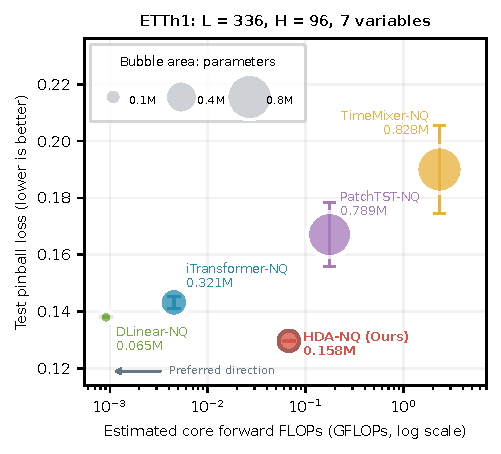
\includegraphics[width=\columnwidth]{figures/efficiency_bubbles.pdf}
\caption{Parameter--accuracy tradeoff on ETTh1 at $H=96$.}
\Description{A bubble plot compares five models by estimated forward FLOPs, test pinball loss, and trainable parameter count. HDA-NQ has the lowest mean pinball and the second-smallest parameter count.}
\label{fig:complexity}
\end{figure}
Figure~\ref{fig:complexity} compares forecasting accuracy, model size, and estimated computation on ETTh1 at $L=336$ and $H=96$. Bubble area denotes trainable parameters, and pinball is the three-seed mean with sample-standard-deviation error bars. Computation is estimated for one full seven-variable input window. HDA-NQ uses 157,960 trainable parameters, compared with 788,732 for PatchTST-NQ, 828,233 for TimeMixer-NQ, and 320,750 for iTransformer-NQ. DLinear-NQ is smaller at 64,718 parameters. Thus, the observed accuracy does not require the largest parameter budget, although the architectures have different tuning histories.

HDA-NQ requires approximately 0.0672 GFLOPs per forward pass under this accounting, with a multiply--add counted as two operations. DLinear-NQ and iTransformer-NQ require less computation, while PatchTST-NQ and TimeMixer-NQ require more. The estimates include sampled attention and key/value interpolation in HDA-NQ, but exclude normalization, nonlinear activations, softmax, miscellaneous elementwise operations, and memory indexing or copying. They support a parameter--accuracy comparison in this setting, not a training-speed or memory-efficiency claim.


\subsection{Prediction and Calibration Analysis}
\begin{figure}[t]
\centering
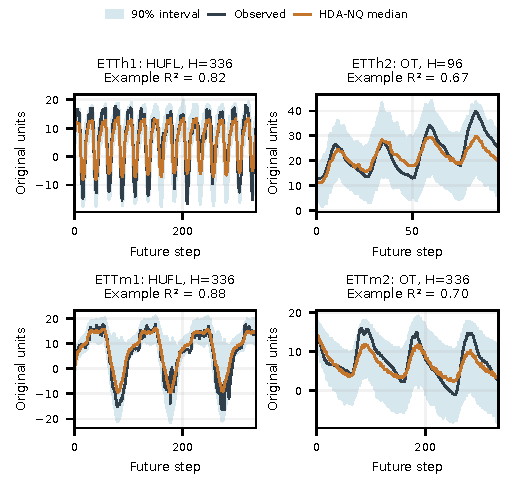
\includegraphics[width=\columnwidth]{figures/dataset_forecasts.pdf}
\caption{Example forecasts and 90\% prediction intervals on the four ETT datasets.}
\Description{Four panels show observed values, predicted medians, and 90 percent intervals for one complete forecast on each ETT dataset.}
\label{fig:forecasts}
\end{figure}
Figure~\ref{fig:forecasts} shows one favorable example per ETT dataset at seed 2024, using $H=96$ on ETTh2 and $H=336$ elsewhere. Within each dataset, we select the highest within-window $R^2$ among seven variables and 21 uniformly spaced test windows. The horizon choices follow qualitative inspection, rather than a matched-horizon comparison. Complete forecasts and 90\% intervals are plotted in original units without smoothing. These selected examples illustrate attainable fit rather than population-average performance and complement the full-test metrics.

\begin{figure}[t]
\centering
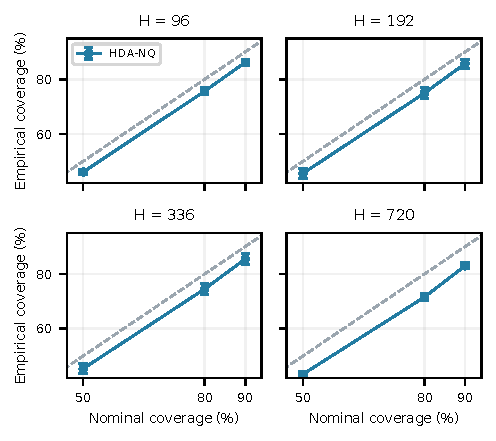
\includegraphics[width=\columnwidth]{figures/revised_calibration.pdf}
\caption{Empirical versus nominal interval coverage on ETTh1.}
\Description{Four panels show HDA-NQ empirical versus nominal coverage at all four prediction lengths.}
\label{fig:calibration}
\end{figure}
Figure~\ref{fig:calibration} compares empirical coverage with nominal 50\%, 80\%, and 90\% levels. Points and error bars show the mean and sample standard deviation over three seeds; the diagonal denotes nominal coverage. The same frozen HDA-NQ configuration is used across prediction lengths. Its empirical 90\% coverage is approximately 86.21\%, 85.72\%, 85.45\%, and 82.97\% as $H$ increases. Figure~\ref{fig:calibration} therefore does not support a calibration-improvement claim. No test-fitted interval widening is applied.

\begin{figure}[t]
\centering
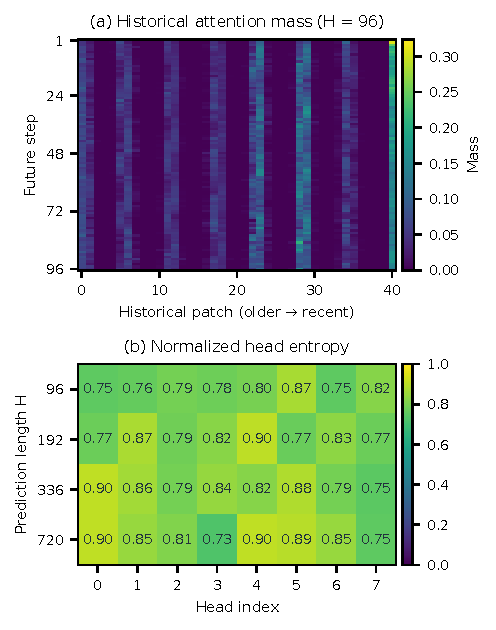
\includegraphics[width=\columnwidth]{figures/revised_attention.pdf}
\caption{ETTh1 attention diagnostics: (a) historical attention mass; (b) normalized head entropy.}
\Description{A historical attention-mass map and a head-entropy heatmap show learned retrieval behavior and diversity across prediction lengths.}
\label{fig:diagnostics}
\end{figure}
Figure~\ref{fig:diagnostics}(a) shows interpolated attention mass averaged over eight heads for a fixed high-fit ETTh1 HUFL case at $H=96$, selected from a separate first/middle/last-window diagnostic set. Each sampled weight is distributed to its two interpolation neighbors, so each future-step row sums to one after head averaging. Panel (b) reports normalized head entropy averaged over three fixed windows, seven variables, future steps, and three seeds. These diagnostics describe retrieval behavior rather than causal feature attribution or full-test population performance; retrained component comparisons assess forecast contribution.

\subsection{Limitations}
The current comparison includes seven benchmark datasets. The remaining settings on Traffic, Weather, Electricity await complete model and seed groups. Four ETT series are related benchmarks, so their results alone do not establish generalization to all domains.
 The final-structure ablations are restricted to ETTh1; their conclusions are not automatically transferable to every dataset. Three seeds describe limited training variability, not statistical significance. Short validation screens can miss slower configurations, and repeated validation use introduces selection optimism. Models have different capacities and tuning histories, and the dataset-specific epoch caps do not establish convergence.

Independent variable processing can miss cross-variable predictive information. Positive gaps exclude exact quantile ties in real arithmetic, and seven marginal quantiles do not define a joint distribution. Undercoverage, especially at long horizons, and imperfect extreme-change prediction remain unresolved. We make no end-to-end efficiency claim from asymptotic sampling cost or shared-GPU training times.


\section{Conclusion}
HDA-NQ combines future-step queries, bounded deformable historical retrieval, a common historical correction, and structurally ordered quantile outputs. The completed comparisons on five benchmark datasets favor the proposed model in 15 of 17 dataset--horizon settings under the stated common-head adaptation and validation budget. ETTh1 component experiments support learned positions and horizon identity, while the correction exhibits a tradeoff between quantile fit and local-variation error. These results do not establish superiority under matched hyperparameter searches. Non-crossing outputs still exhibit undercoverage, and cross-variable modeling and validation-only calibration remain useful directions. Conclusions about Traffic, Weather, and Electricity await their complete experimental matrices.

\bibliographystyle{ACM-Reference-Format}
\begingroup
\balance
\interlinepenalty=10000
\bibliography{references}
\endgroup
\end{document}
